\subsection{Xtext Overview}

This overview will give you a rough idea about what
Xtext\footnote{\url{http://www.xtext.org}} is all about. We will then dive into
the details and work on a small project.

In a nutshell, Xtext is a workbench to create and work with textual
domain-specific languages (DSLs). It comes as a feature (set of plugins) to the
popular Eclipse IDE.

The first thing you will want to do is to create your own domain-specific
language (DSL) and specify a \emph{grammar} for it. The grammar file is a plain
text file with ``\texttt{.xtext}'' filename extension, and the grammar within is
defined with a BNF like syntax. While you can use any text editor to modify it,
Xtext gives you a specialized editor for grammar files. It is aware of the Xtext
language, gives you syntax coloring, code completion, and more. To get a first
impression see the screenshot of the Xtext grammar file, opened with the Xtext
grammar editor, below. It is not required to fully understand the content yet,
this will be discussed in the next chapter in detail.

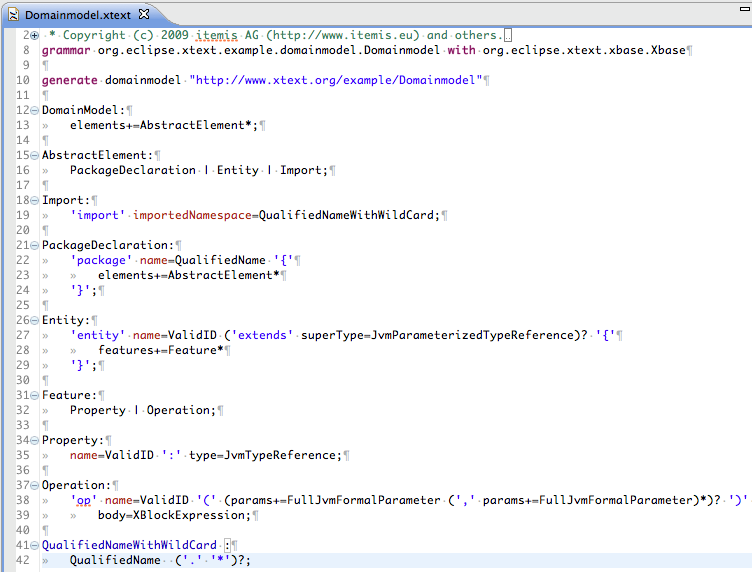
\includegraphics[width=16cm]{images/intro/overview-xtext-grammar.png}

The aforementioned example DSL allows you to define entities like ``Person'',
``Car'', ``Book'', and so on.
An entity has properties, e.g. a
Person has a name, a gender, and a date of birth. A Book has a title, one or
more authors, and an ISBN number.

A textual DSL model could look like this, but you could also imagine other
syntaxes:
\begin{lstlisting}
entity Person {
  name : String
  gender : m
  birthday : Date
}

entity Book {
  title: String
  authors: Person[]
  isbnNumber: String
}
\end{lstlisting}

Note that the Property \texttt{authors} is of type \texttt{Person}, so there can
be references between entities. In the Xtext grammar file you specify how you
want to define entities and their properties.

Once you have completed your language, you can do that: define some entities,
say ``Book'' and ``Person'', together with their respective properties and with
proper references between them. The nice thing is that Xtext not only gives you
a syntax-driven editor for editing grammar files. Additionally it generates an
editor that is specific to the language you have defined. It knows about your
language's keywords and where to place them, it knows about all the syntactical
constructs you have made up in your grammar, it includes all the nice stuff like
syntax coloring, code completion, validation, and more. For example, if you are
at some point where a reference to another entity must be inserted, your DSL
editor shows you all the references that would be valid here -- according to
your language rules -- and lets you choose among them. All in all, using the DSL
editor generated by Xtext, it is quite easy to establish a text file that adhers
to your DSL.

Depending on your language's type, you could call this text file e.g. a model, a
document, a program, or whatever. We will refer to DSL files here as
\emph{models} (files).

Consider now that you have created a model. What can you do with it? A typical
requirement is to generate an implementation of it in a language like Java, C++,
or XML. Or a graphical representation. Or something quite different. This is
where code generation comes in. Xtext creates a skeleton
code generator for you. Typically you use that code generator as a starting
point to produce e.g. Java source code, documentation in, say, DocBook or Wiki
format, overview graphics using GraphViz, or any other stuff you need. Xtext
offers special support for textual output formats, but it is also possible to
generate binaries.

This was only a short outline of some prominent Xtext aspects. It is by far not
everything Xtext can do for you, but it should suffice for now. The next
chapters will show you in more detail how to work with Xtext.
